\section{图表}

\begin{genbox}{函数图像示例}
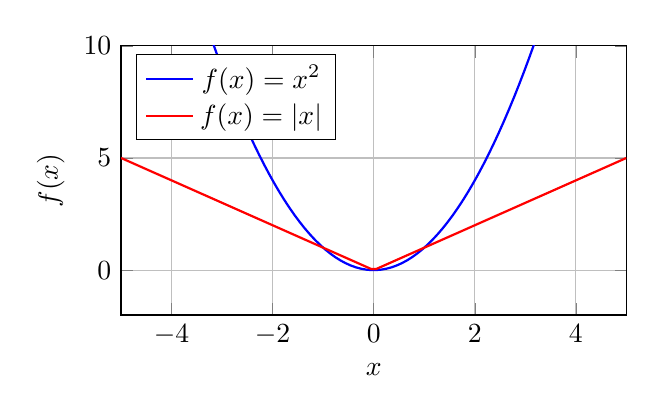
\begin{tikzpicture}
\begin{axis}[
    width=8cm,
    height=5cm,
    xlabel={$x$},
    ylabel={$f(x)$},
    grid=major,
    xmin=-5, xmax=5,
    ymin=-2, ymax=10,
    legend pos=north west,
]
\addplot[blue, thick, samples=100] {x^2};
\addlegendentry{$f(x) = x^2$}
\addplot[red, thick, samples=100] {abs(x)};
\addlegendentry{$f(x) = |x|$}
\end{axis}
\end{tikzpicture}
\end{genbox}

\begin{genbox}{三角函数图像}
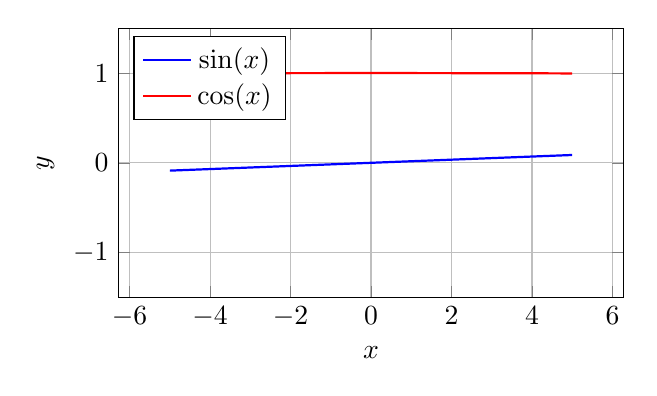
\begin{tikzpicture}
\begin{axis}[
    width=8cm,
    height=5cm,
    xlabel={$x$},
    ylabel={$y$},
    grid=major,
    xmin=-6.28, xmax=6.28,
    ymin=-1.5, ymax=1.5,
    legend pos=north west,
]
\addplot[blue, thick, samples=100] {sin(x)};
\addlegendentry{$\sin(x)$}
\addplot[red, thick, samples=100] {cos(x)};
\addlegendentry{$\cos(x)$}
\end{axis}
\end{tikzpicture}
\end{genbox}

\begin{genbox}{指数函数图像}
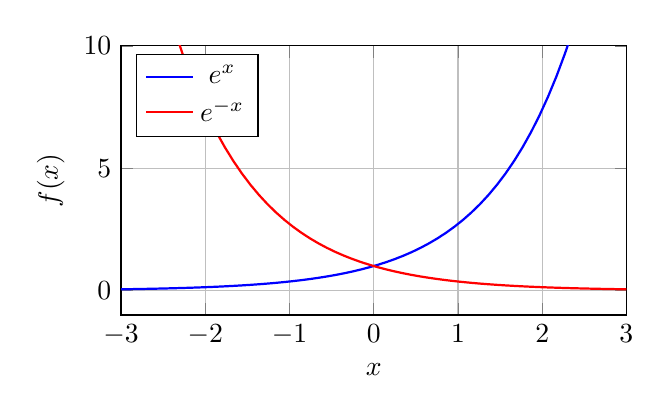
\begin{tikzpicture}
\begin{axis}[
    width=8cm,
    height=5cm,
    xlabel={$x$},
    ylabel={$f(x)$},
    grid=major,
    xmin=-3, xmax=3,
    ymin=-1, ymax=10,
    legend pos=north west,
]
\addplot[blue, thick, samples=100] {exp(x)};
\addlegendentry{$e^x$}
\addplot[red, thick, samples=100] {exp(-x)};
\addlegendentry{$e^{-x}$}
\end{axis}
\end{tikzpicture}
\end{genbox}